\label{prototype}
For the simulation model NetLogo was used as a simulation tool whereas the random data was generated with R.
In the following, the data model, the R script, the GUI and code from Netlogo will be described.
\subsection{Data model}
According to the problem description we defined a generic data model for every individual.
This data model is valid for the disco example, the university and labour market example, and contains the following attributes:
\begin{itemize}
	\item id: unique object identifier
	\item name: object name (e.g. male1 or female1)
	\item maxMatchesInt: integer value representing the maximum number of matchings for this individual (e.g. in the disco example each person is maximally matched with one other person)
	\item sideInt: integer helper variable assigning an individual to one of the two participant groups
	\item partnerList: list of identifiers of the partners, ordered according to the preference of an individual
	\item rankList: list of ranks (values between 1 to 0) for the partners from the partnerList; the list is ordered from highest to lowest preferences.
	If the value is equal to 1 this partner is a perfect match.
	\item hasProposedToList: list of identifiers representing the individuals to which an individual has proposed
	\item gotProposedByList: list of identifiers representing the individuals from which an individual received proposals.
	The gotProposedByList is only valid for one iteration.
	\item tmpMatchList: list containing the identifiers of individuals to whom a temporary match was established
	\item activeFlag: boolean value stating if an individual is matched or not respectively if the individual gave up (they already proposed to all individuals from the partnerList but only received rejections)
\end{itemize}

\subsection{Data generation}
In order to generate data for the disco example, the statistical computing language R\footnote{Available at \url{https://www.r-project.org/}, accessed April 28, 2016} has been used. 
This generates a CSV list, which is then read from NetLogo. 
The script accepts the following parameters:
\begin{itemize}
	\item seed: integer value, which is used as a seed by the number generator. The default value is 123.
	\item numberOfMen: integer value representing the number of men which should be created. The default value is 10.
	\item numberOfWomen: integer value representing the number of women which should be generated. The default value is 10.
	\item pickyLower: float value between 0 and 1 representing the lower bound which will be used in order to generate a number that represents how picky a person is. The value 0 means accepts every possible match, the value 1 excepts none.
	\item pickyUpper: float value between 0 and 1 representing the upper bound which will be used in order to generate a number that represents how picky a person is. The value 0 means excepts every possible match, the value 1 excepts none.
\end{itemize}

The script can be called as follows from the command line: 
\begin{verbatim}
Rscript initDisco.R 123 10 10 0 0
\end{verbatim}

The script generates a CSV which looks as follows:
\begin{verbatim}
"";"id";"name";"maxMatchesInt";"sideInt";"partnerList";"rankList"
"1";1;"male1";1;1;"13#18#14#17#16#11#20#19#12#15";"0.96#0.95#0.9#0.68#0.57#0.45#0.33#0.25#0.1#0.04"
...
"11";11;"female1";1;2;"3#9#5#4#10#8#2#1#6#7";"0.92#0.82#0.7#0.67#0.48#0.41#0.35#0.25#0.22#0.05"
\end{verbatim}

\subsection{GUI}
One of the main goals in the design phase was to keep the GUI simple and clear.
The GUI was structured in two main parts - the control and the information section.
\begin{figure}[H]
  \caption{The control section for the disco example}
	\label{fig:control-disco-gui}
  \centering
    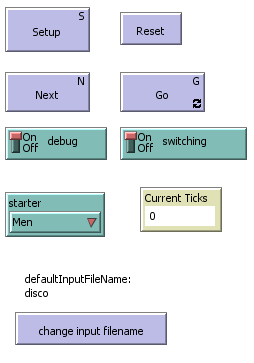
\includegraphics[width=0.5\textwidth]{netlogo-controls}
\end{figure}
Figure~\ref{fig:control-disco-gui} shows the control section in the GUI. 
With the buttons Setup and Reset the simulation model can be initialized or reset after a simulation run.
The button Next advises the program to perform one simulation step, if Go is activated the simulation continues a termination criterion is met.
In the disco example the main termination criterion is if every every proposing person is already matched to another person. 
Another criterion for termination is if the proposing person already proposed to every person in his partnerList but got rejected every time.
The debug-switch enables or disables debug messages which are printed during the simulation run.
The speed of a simulation run can be increased if the debug-switch is set to Off.
The second switch, switching, controls, if the two parties propose to each other alternatively (On) or if only one party proposes to the other one (Off).
With the drop-down list starter the user can determine which party starts proposing.
The reporting box Current Ticks shows the current number of simulation steps.
The button change input filename raises a dialogue box where the user can enter the filename of an input file which shall be used in the simulation.
Together with the number of ticks the filename will also be used as the name for the CSV export file.
\begin{figure}[H]
  \caption{The information section for the disco example}
	\label{fig:info-disco-gui}
  \centering
    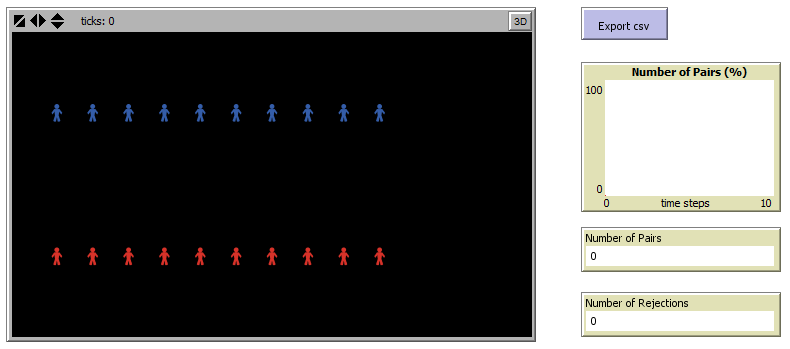
\includegraphics[width=0.8\textwidth]{netlogo-information}
\end{figure}
Figure~\ref{fig:info-disco-gui} shows the information section of the disco example GUI. 
All created humans are shown in the world area. 
Men are coloured blue and women are red.
On setup of the simulation the proposing site is shown in the top row. 
As soon as two people are matched their colour changes to green and a link between the two is established.
If a couple is divorced the link is removed and the colour changes back to the original one.
The plot named Number of Pairs (\%) illustrates at each point in time how many of the possible couples exist. 
If the simulation contains 10 men and women and currently 4 couples exist, the plot shows that 40\% are matched.
The reporting box Number of Pairs shows the absolute number of couples.
The other reporting box, Number of Rejections, indicates how many couples were divorced over time.
With the button Export csv the current properties of all humans are exported to a csv file.
The filename is a combination of the input filename and the current number of ticks.

\subsection{Netlogo code}
